\documentclass[12pt,a4paper]{report}

\usepackage[dutch]{babel}
\usepackage{colortbl}

\usepackage{graphicx}
\DeclareGraphicsExtensions{.pdf,.png,.jpg}

\usepackage{textcomp}

\usepackage{geometry}
\geometry{a4paper,total={180mm,247mm},left=20mm,top=20mm}

%% Use no serif font for text, courier for commands
\newcommand*{\myfont}{\fontfamily{lmss}\selectfont}
\newcommand*{\monofont}{\fontfamily{pcr}\selectfont}

\setlength{\parindent}{0pt}

\begin{document}

\myfont

\title{
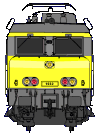
\includegraphics[scale=1.0]{images/rcu_logo}
\makebox[\linewidth]{\rule{\textwidth}{0.4pt}}
Railclub Utrecht
\vfill
Normen H0 groep\\
\makebox[\linewidth]{\rule{\textwidth}{0.4pt}}
\vfill
\small
\author{Peter Mansvelder}
\begin{tabular}{| l | l |}
\hline
\cellcolor[gray]{0.84}Titel & Normen H0 groep Railclub Utrecht\\
\hline
\cellcolor[gray]{0.84}Auteur & Peter Mansvelder\\
\hline
\cellcolor[gray]{0.84}Eigenaar & Marc Timmermans / Peter Mansvelder\\
\hline
\cellcolor[gray]{0.84}Versie & 3.0\\
\hline
\cellcolor[gray]{0.84}Versiedatum & \today\\
\hline
\cellcolor[gray]{0.84}Status & Concept\\
\hline
\end{tabular}
}

\maketitle

\tableofcontents

\chapter{Opbouw document}

\section{Documentoverzicht}

Hoofdstuk 1 geeft de inhoud van dit document.

Hoofdstuk 2 geeft een korte inleiding tot het systeem.

Hoofdstuk 3 beschrijft de benodigdheden.

Hoofdstuk 4 beschrijft de uit te voeren werkzaamheden.

Hoofdstuk 5 beschrijft het fallback scenario.

Hoofdstuk 6 bevat het communicatieplan.
\section{Afkortingen en begrippen}
\begin{tabular}{| l | l |}
\hline
\rowcolor[gray]{0.84}Afkorting & Omschrijving\\
\hline
DCC & Digital Control Systeem, het NMRA-standaard digitale systeem voor modeltreinen\\
\hline
MM & Motorola, het door M\"{a}rklin gebruikte digitale systeem\\
\hline
\end{tabular}

\chapter{Inleiding}

M-trak is een modulair systeem voor half nul met een middenrail, waarbij de beide spoorstaven elektrisch gescheiden zijn. Bij de RailClub Utrecht wordt dit systeem gebruikt om zowel 2- als 3-rail systeem rollend materieel te laten rijden.

\section{Systeemnormen}

De systeemnormen van M-trak bestaan uit:
\begin{itemize}
\item Het gebruikte (digitale) systeem
\item Een genormaliseerde kopkant van de modules;
\item Een minimum boogstraal van de hoofdbaan;
\item Het type wissels dat gebruikt kan worden in de hoofdbaan;
\item De hoogte van de sporen t.o.v. de vloer.
\end{itemize}

De afspraken zijn als volgt:
\\

\begin{tabular}{| l | l |}
\hline
\cellcolor[gray]{0.84}Digitaal Systeem & Gecombineerd DCC/Motorola\\
\hline
\cellcolor[gray]{0.84}Lengte standaard module & Aanbeveling max. 1200 mm\\
\hline
\cellcolor[gray]{0.84}Breedte standaardmodule & 600 mm\\
\hline
\cellcolor[gray]{0.84}Hoogte standaardmodule & Voorzijde 120 mm, Spoordijk 150 mm hoog\\
\hline
\cellcolor[gray]{0.84}Hoogte bovenkant spoorstaaf t.o.v. de vloer&1200 mm $\pm$ 25 mm\\
\hline
\cellcolor[gray]{0.84}Aantal sporen&Twee\\
\hline
\cellcolor[gray]{0.84}Hartafstand van de sporen K-Rail 2200 serie&57 mm\\
\hline
\cellcolor[gray]{0.84}Minimum boogstraal binnenboog&Grote cirkel 1 van M\"{a}rklin, radius 553,9 mm\\
\hline
\cellcolor[gray]{0.84}Minimum boogstraal buitenboog&Grote cirkel 2 van M\"{a}rklin, radius 618,5 mm\\
\hline
\cellcolor[gray]{0.84}Type wissels&2272, 2273, 2275, 22715 en 22716\\
\hline
\cellcolor[gray]{0.84}Materiaal voor de constructie van de modulen&Multiplex 12 mm\\
\hline
\cellcolor[gray]{0.84}Constructie&Open raambouw methode\\
\hline
\cellcolor[gray]{0.84}Afstand tussenschotten&Maximaal 400 mm\\
\hline
\cellcolor[gray]{0.84}Kleur voorzijde&Schoolbordenverf, zwart\\
\hline
\cellcolor[gray]{0.84}Poten&Volgens tekening, in hoogte te verstellen tot $\pm$ 25 mm\\
\hline
\cellcolor[gray]{0.84}De bovenleiding&Sommerfeldt\\
\hline
\end{tabular}

\chapter{Modules}
Het systeem is opgebouwd uit modules. Er zijn verschillende modules mogelijk:

\section{De rechte module met spoordijk}
De rechte module voor de vrije baan, deze kan een lengte hebben van 580 mm, 890 mm of de ''standaard'' lengte van 1200 mm.
Andere lengtematen zijn toegestaan, alleen moet dan rekening gehouden worden met de rijdraadlengte die gebruikt wordt. De rijdraad bij de overgang van de modulen is 270mm lang en op de modulen 310mm.
Bij een standaardmodule is die 3 keer 310mm + 270mm geeft samen de 1200mm lengte.

Een standaard module met spoordijk bestaat uit twee hoofdbestanddelen: 
\begin{itemize}
\item De bovenbouw die ook wel de bak wordt genoemd.
\item Vier afneembare poten, deze dienen in hoogte verstelbaar te zijn.
\end{itemize}
Meer info voor de constructie van deze poten, vindt u onder het kopje ''opbouw van de poten''.

De bovenbouw van de module wordt samengesteld uit twee gelijke kopschotten en twee zijkanten van 120 mm hoog en 1200 mm lang. Daar tussen komen nog twee tussenschotten.
Tussen de kopschotten wordt de ondergrond voor de baan, het trac\'{e}', aangebracht. Het trac\'{e} rust op de tussenschotten. 

Hierna wordt het neopreen band tussen de kopschotten op de ondergrond voor het trac\'{e}' aangebracht. De bovenkant van het neopreenband zit gelijk met de bovenkant van de kopschotten, zie figuur 1.

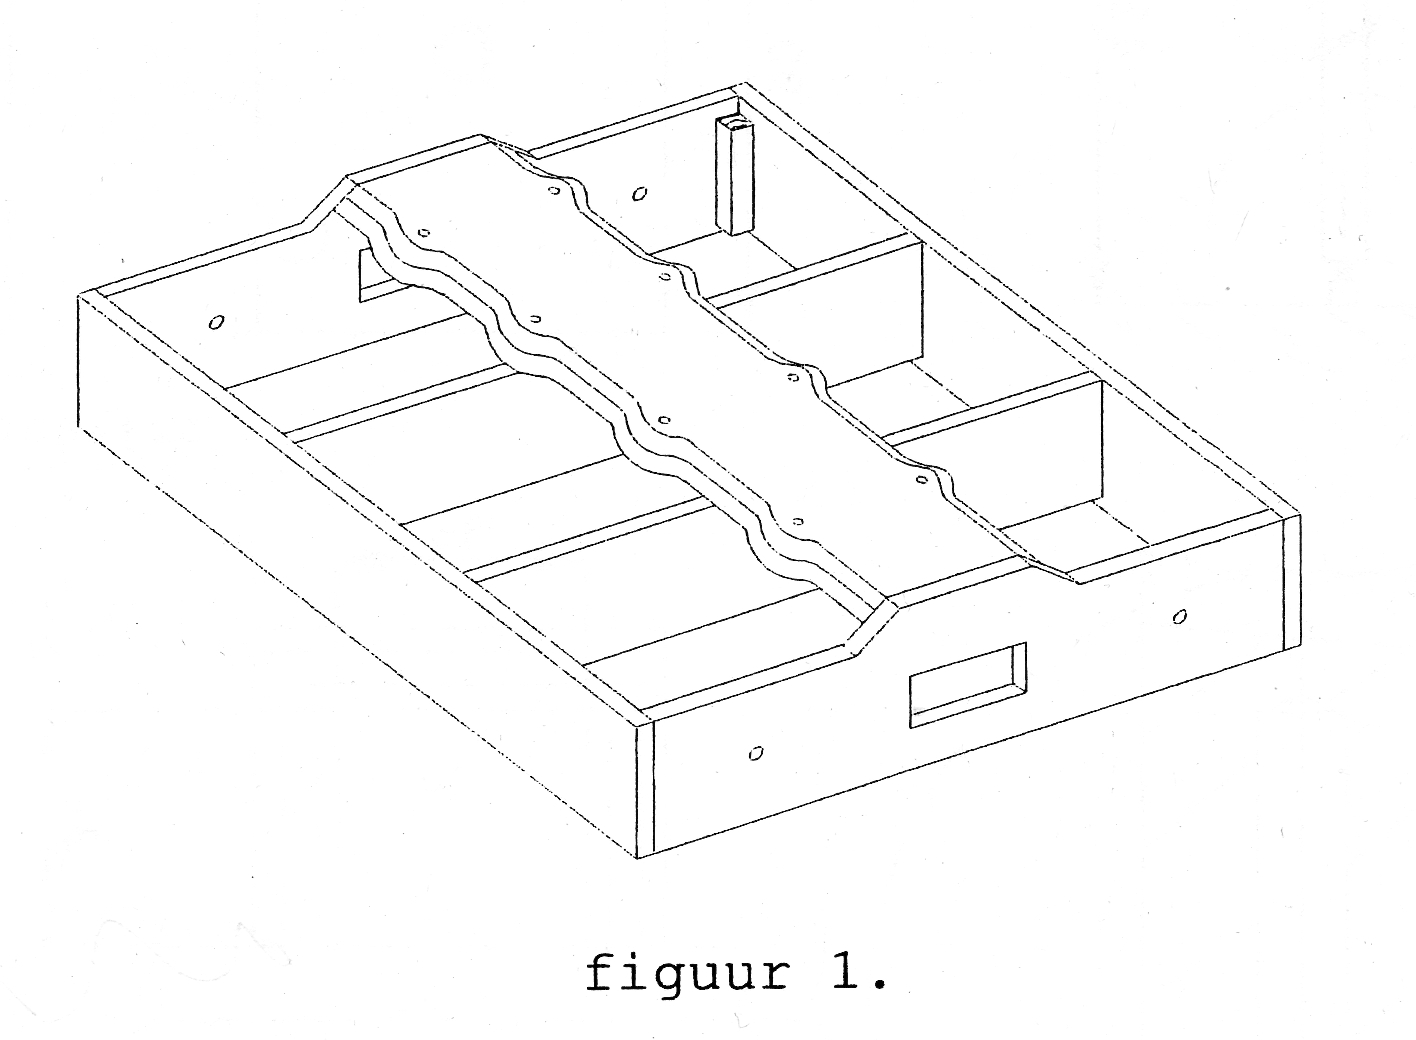
\includegraphics[scale=0.2]{images/rcu_figuur1}

De kopschotten dienen nog wel in de vorm van het neopreen band te worden gevijld. 

Nu trekken we eerst een hartlijn, in het midden van het spoortracé, van het ene kopschot naar het andere. Dit moet nauwkeurig worden gedaan, omdat vanuit deze lijn de plaats wordt bepaald waar de rails komen te liggen.
Het leggen van de rails wordt later uitgebreid behandeld.

Nu worden de gaten geboord waar later de masten voor de bovenleiding in geplaatst worden. 
Plaatsen van 3 mm ringen niet vergeten (dikte neopreen).
Hierna kan de moer die onderaan de mast zit ''vast'' worden gedraaid.

\subsection{Opbouw poten}
De poten voor de baan zijn allemaal op dezelfde wijze opgebouwd en kunnen zonder problemen met elkaar verwisseld worden. In de bakken zit een standaard constructie waarin de poten geschoven kunnen worden en vastgezet, zie figuur 2.

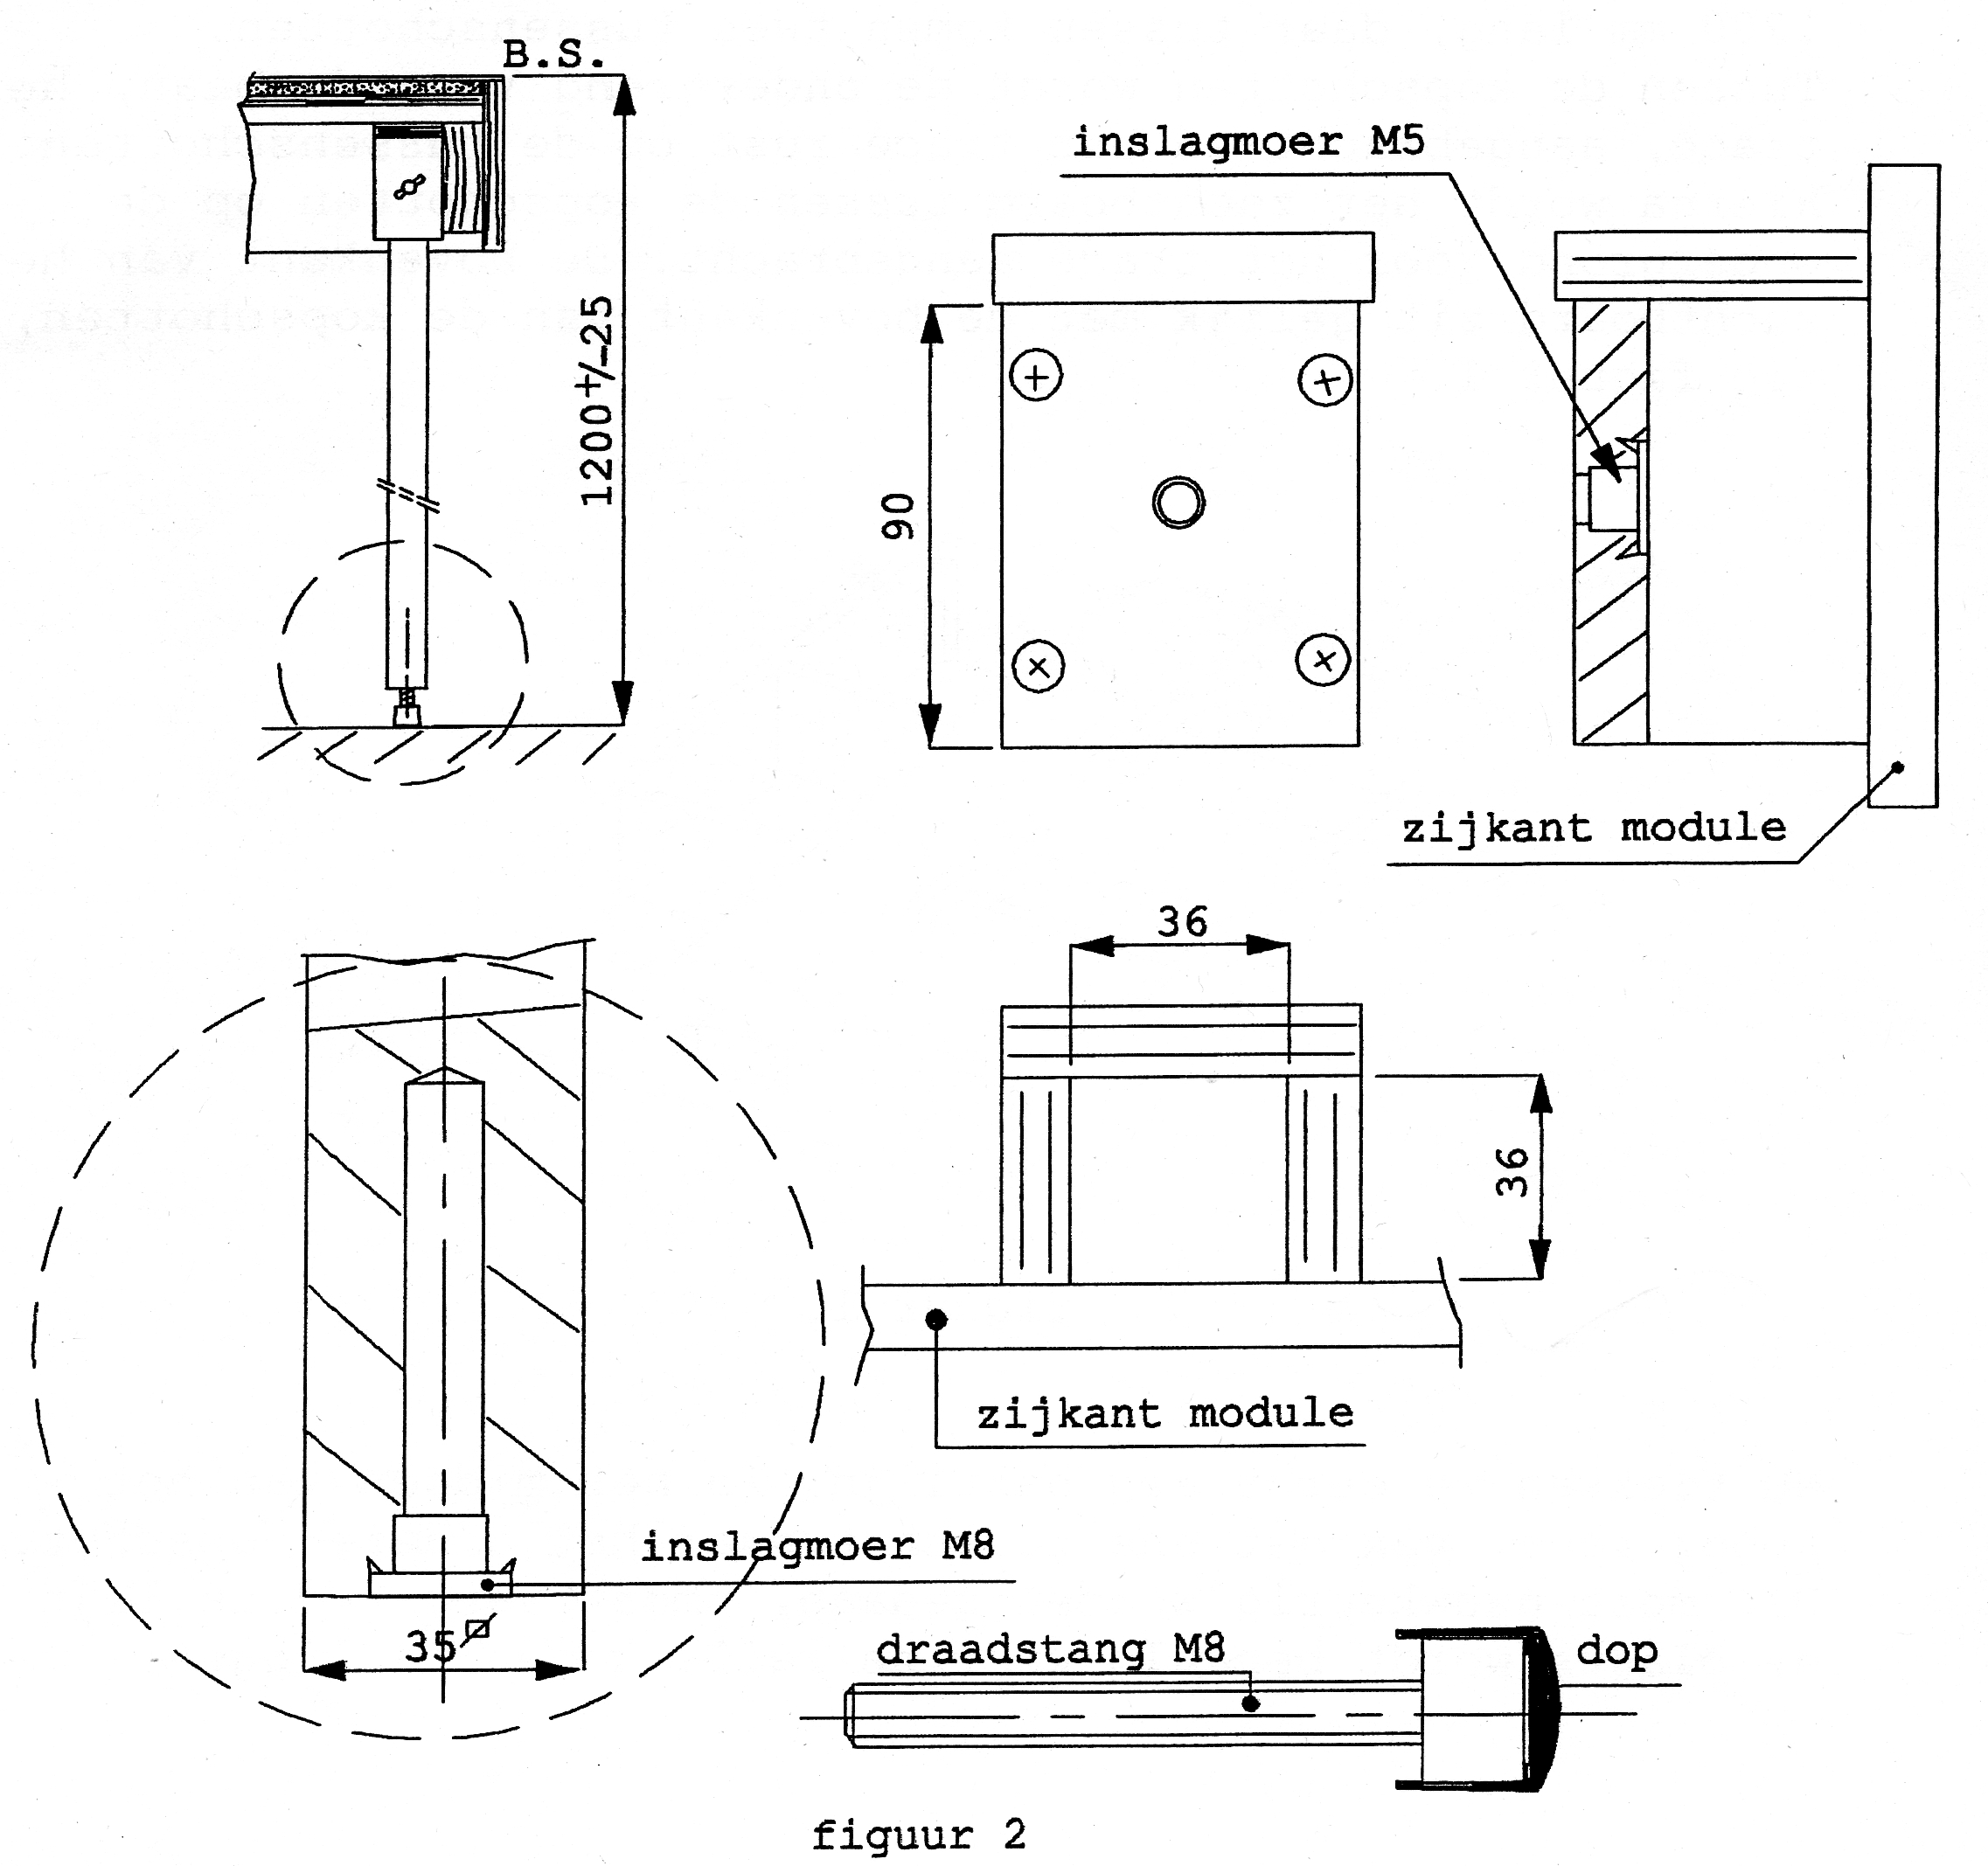
\includegraphics[scale=0.2]{images/rcu_figuur2}

De poten kunnen zowel van hout als metaal gemaakt worden en zijn vierkant De poot heeft een dikte van 35 mm en de schacht waarin hij schuift 36 mm. Hierdoor kan de poot altijd makkelijk in en uit genomen worden. Om te voorkomen dat de poot er op het verkeerde moment uitschuift wordt deze met een vleugelboutje vastgezet. Om te voorkomen dat dit vleugelboutje steeds dieper het hout wordt ingedraaid wordt op die plaats een metalen plaatje aangebracht. Zie figuur 3.

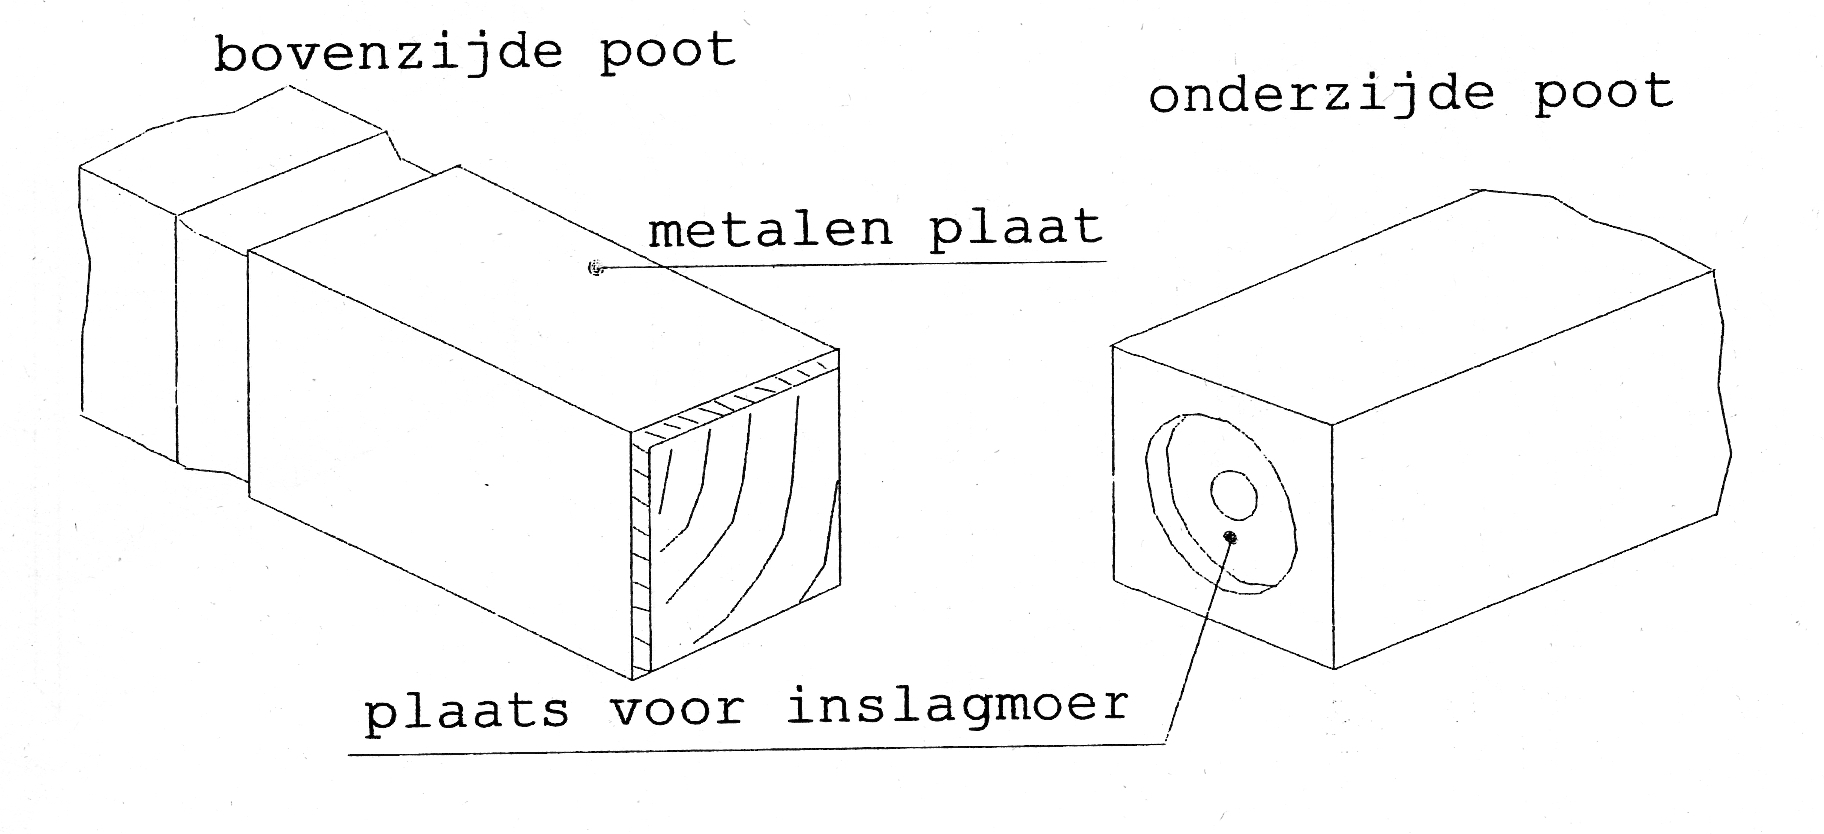
\includegraphics[scale=0.2]{images/rcu_figuur3}

De draadstang met daarop een metalen schijf,  met een kunststof dop er overheen, moet voldoende lang zijn om een hoogteverstelling van 50 mm mogelijk te maken.

\section{De rechte module zonder spoordijk}
Een module zonder spoordijk, met 2 sporen die aan een kant van de module worden gelegd, zodat er meer ruimte is voor scenery aan de achterkant. Dit zijn de oude jeugdmodules.

\section{Overgangsmodules}
Overgangsmodules tussen de twee verschillende soorten modules (met en zonder spoordijk).

\section{De hoekmodule}
De standaard hoekmodule heeft een hoek van $45$\textdegree. Eventueel is een andere hoek ook mogelijk.
Zowel bij de rechte als bij de hoek module is het kopschot uitgevoerd volgens het standaard profiel, zie hiervoor de tekeningen!

Het maken van een standaard hoekmodule is lastiger dan van een rechte module. Een hoekmodule hoeft niet de standaard vorm of hoek te hebben, maar wel het standaard kopschot.

Bij de beschrijving hierna wordt uitgegaan van een standaard hoekmodule. Deze module heeft een hoek van 450 De grootste lengte van de bak is 875 mm en de kleinste lengte 415 mm. De kopzijde is gelijk aan de standaard kopschotten.
De hoek tussen een kopschot en een zijschot is 22,50. Er zijn twee mogelijkheden om dit te realiseren. Men zaagt een balkje onder een hoek of stukjes multiplex. Zie figuur 4.

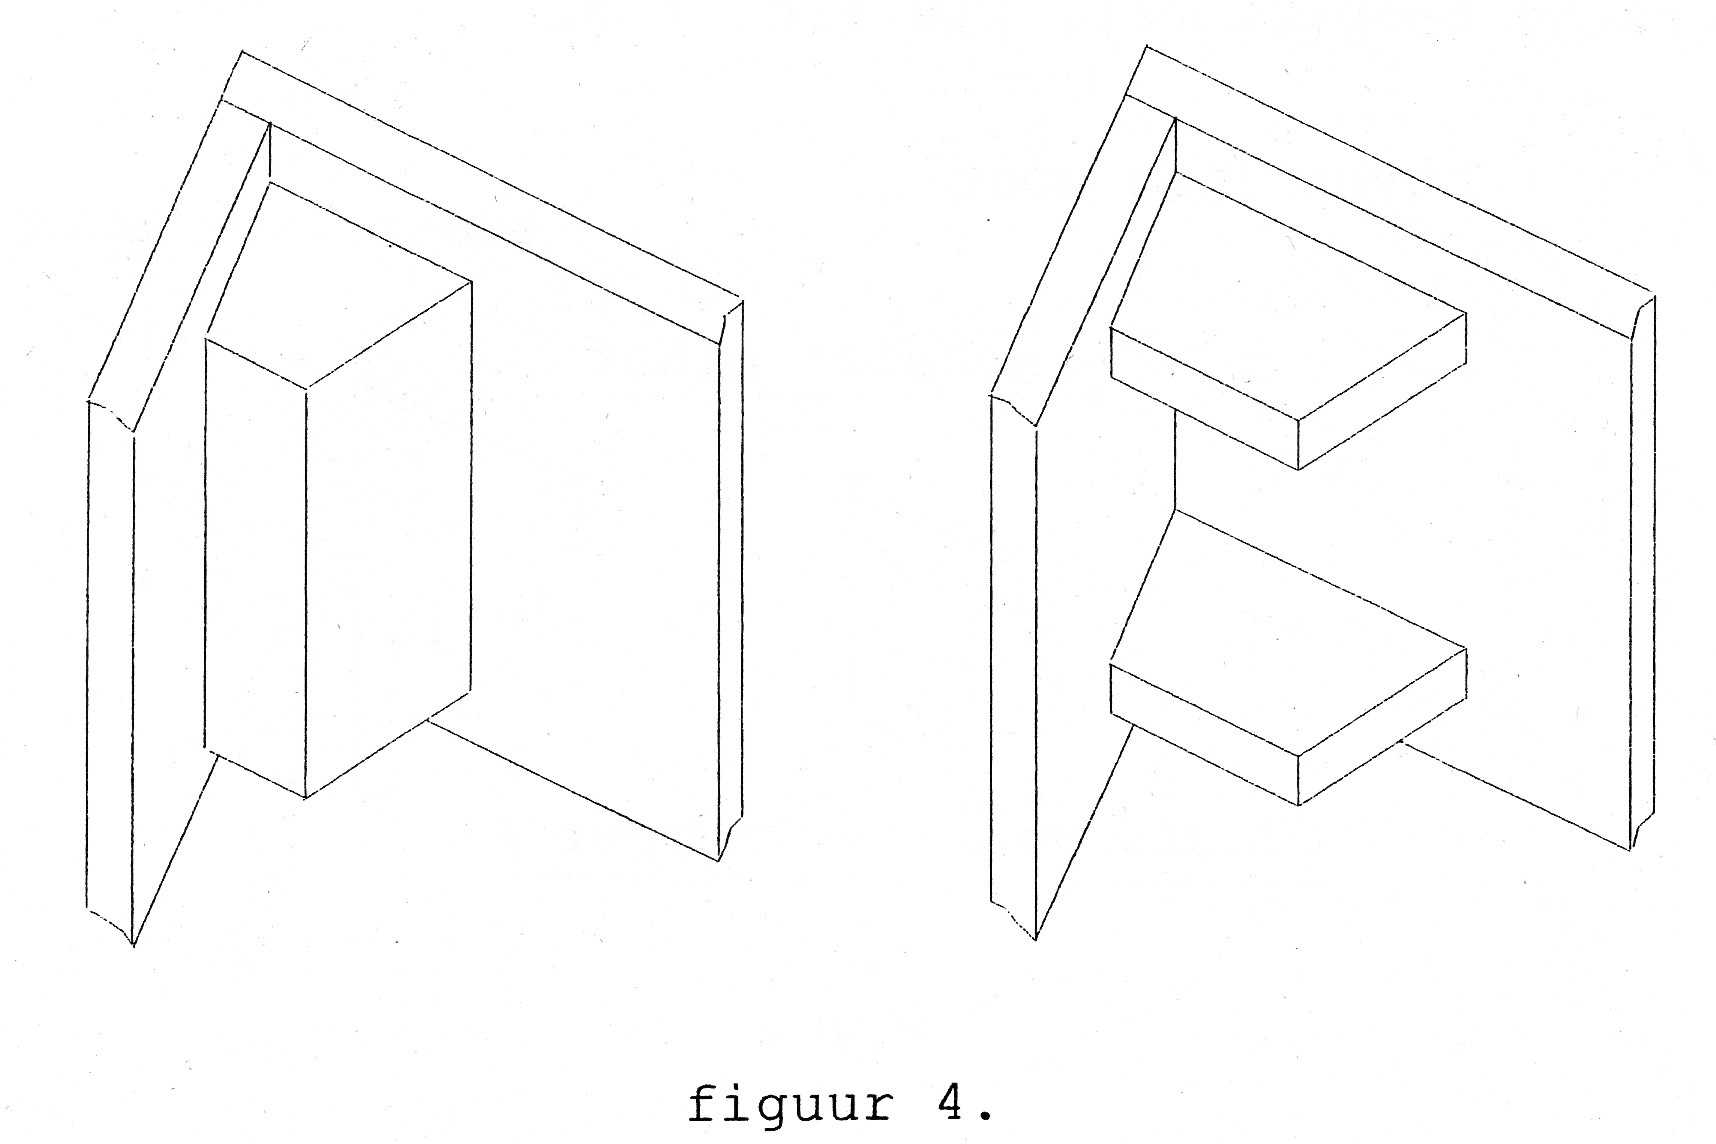
\includegraphics[scale=0.2]{images/rcu_figuur4}

Tegen deze hoekversteviging kan dan de standaard constructie voor de poten bevestigd worden. Hierna wordt de ondergrond van het baantracé bevestigd. Er dient rekening mee gehouden te worden dat de eerste tien centimeter van de rails haaks, t.o.v. het kopschot ligt, en daarna pas de bocht begint. 

De kopschotten dienen nog wel in de vorm van het neopreen band te worden gevijld. 

Hierna wordt het neopreen aangebracht en daarop de rails gelegd. Nu worden de gaten geboord waar later de masten voor de bovenleiding in geplaatst worden. 
Plaatsen van 3 mm ringen niet vergeten (dikte neopreen).
Hierna kan de moer die onderaan de mast zit ''vast'' worden gedraaid.

\section{De stationsmodules}
Deze bestaan meestal uit meerdere modulen, die altijd op dezelfde wijze aan elkaar gekoppeld worden. Hierdoor hoeft alleen het eerste en het laatste kopschot het standaard profiel te hebben. De tussenliggende kopschotten zijn voor wat betreft de vorm afhankelijk van het sporenplan.

De modules worden opgebouwd van 12 mm dik multiplex. Het beste is om ocum\'{e} triplex te gebruiken. De rails wordt ondersteund door een strook van 8 mm dik multiplex met daarop een 10 mm dikke laag zachtboard of een ander geluiddempend materiaal.
De rest van de module wordt opgebouwd volgens de open raam bouwmethode.

\chapter{Het leggen van de rails}

Het leggen van de rails dient zo nauwkeurig mogelijk te gebeuren! Hierbij wordt gebruik gemaakt van de hartlijn die op de bovenkant van het baantrac\'{e} is aangebracht.
Het hart van de rails ligt op 28,5 mm van de hartlijn. Nu wordt eerst deze hartlijn op het baantrac\'{e} getekend.

\section{Gebruikte rail}
Voor een standaard module van 1200 mm gebruiken we een standaard K-rail flexrail van 900mm (artikelnummer 2205), plus 2 x een vaste lengte van 180mm (artikelnummer 2200). 
\section{Montage}
De flexrail wordt in het midden gemonteerd, en de 2 vaste lengtes worden hieraan gemonteerd en steken dus in eerste instantie aan beide zijden uit. Voor de bevestiging worden de standaard railverbinders gebruikt, en de standaard klemmetjes voor het verbinden van de middenrail. Hierna worden deze laatste klemmetje aan elkaar gesoldeerd:
\begin{itemize}
\item leg de complete constructie plat op een tafel, met de rails aan de onderkant, zodat de metalen strip voor de middenrail boven ligt.
\item Soldeer de lipjes van de midenrail aan beide zijden aan elkaar, zodat er zowel mechanisch als elektrisch een solide verbinding ontstaat.
\item Soldeer minimaal 2 draden aan de middenrail, elk aan een kant van de bak. Gebruik hiervoor een rode draad. Hiervoor moet het metaal worden blootgelegd middels een slijpschijfje (dremel), en als hulpmiddel voor het solderen kan verdund fosforzuur gebruikt worden.
\end{itemize}

Wanneer deze draden zijn vast gesoldeerd wordt de rails op het baantrac\'{e} gelegd en met markeerspelden vastgezet. Deze spelden houden de rails op zijn plaats totdat deze zijn vastgelijmd. Bij de aansluitdraden wordt een klein gaatje geboord en de aansluitdraad door dit gaatje geschoven en strak getrokken. Wanneer de rails nu op de goede plaats ligt worden deze vastgelijmd. Voor het op de goede plaats leggen van de tweede rails maken we gebruik van een schuifmaat. Zie figuur 5.

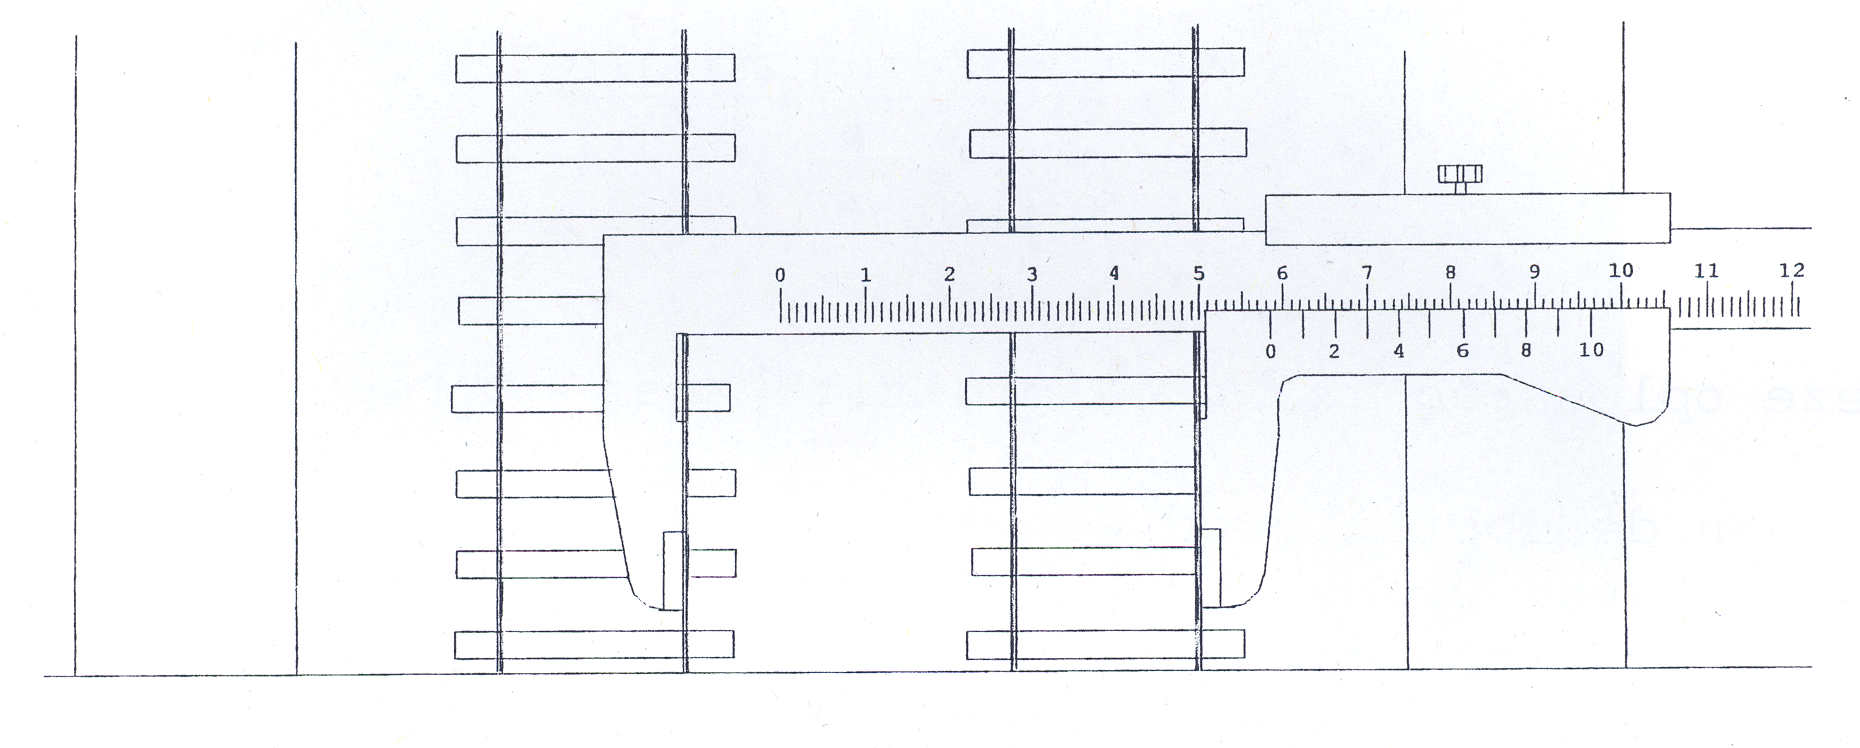
\includegraphics[scale=1.0]{images/rcu_figuur5}

De schuifmaat wordt ingesteld op 57 + 1.3 = 58,3 mm. De 57 mm is de hartafstand van de sporen en de 1,3 mm is de dikte van de spoorstaaf.
Ook de tweede rails wordt voor het leggen eerst voorzien van aansluitdraden alvorens deze wordt vastgelijmd.
Voor een extra stevig`e bevestiging aan het uiteinde wordt er in de laatste dwarsligger aan weerszijde een klein gaatje geboord. Hierdoor drukken we een klein spijkertje dat goed vast komt te zitten in het multiplex van het kopschot. Hiervoor kan ook een markeerspeld gebruikt worden, dan is voorboren niet nodig. Nu kunnen de spoorstaven netjes afgezaagd worden en zodanig afgevijld dat zij precies gelijk met het kopschot eindigen. Als alles goed is gegaan zal het koppelen van twee modules geen problemen geven. Maar om geringe afwijkingen toch nog te kunnen opvangen worden de spoorstaven over een lengte van $\pm$ 15 mm aan de binnenzijde afgeschuind. Zie figuur 6.

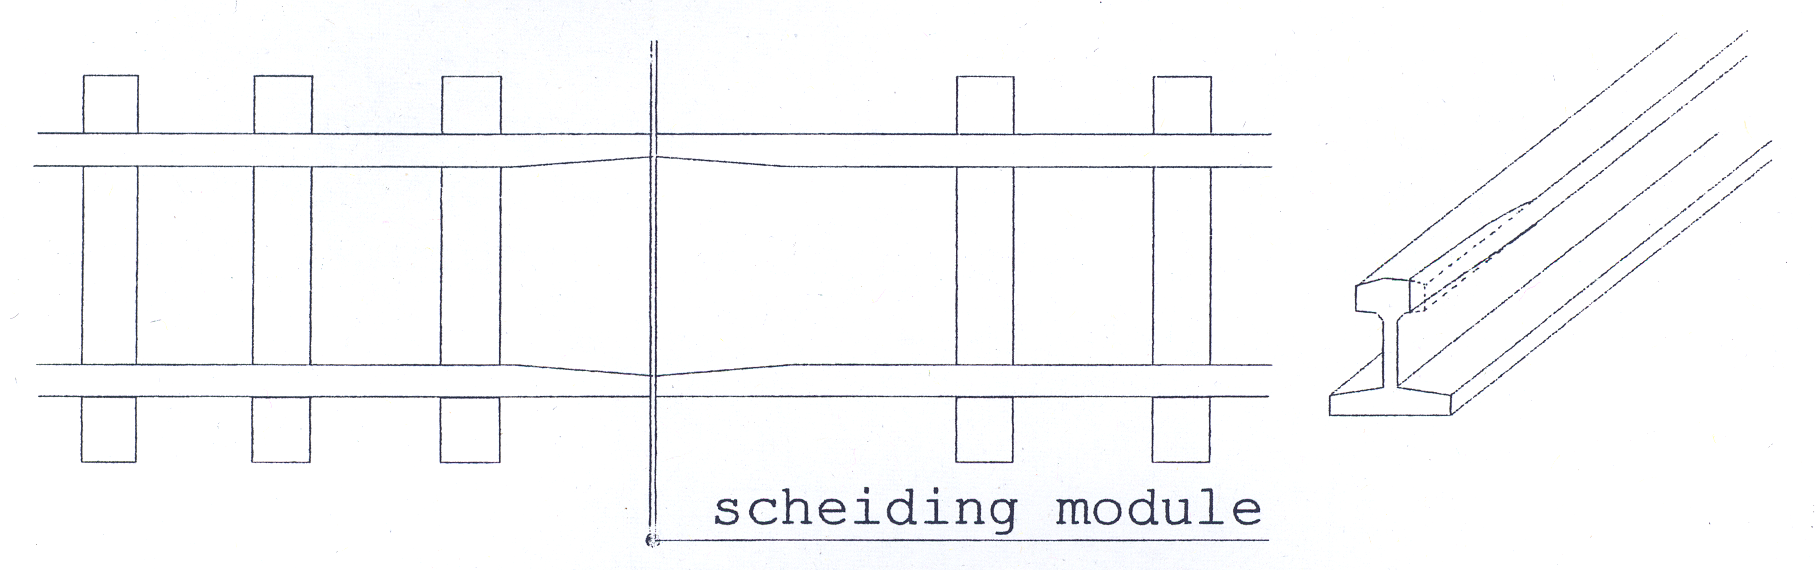
\includegraphics[scale=1.0]{images/rcu_figuur6}

Deze oplossing is in de praktijk zeer betrouwbaar gebleken.

Liggen de spoorstaven goed dan kunnen de draden aan de spoorstaven worden gesoldeerd. Het solderen aan de spoorstaven vraagt enige voorbereiding. Eerst moet, op de plaats waar later gesoldeerd wordt, de spoorstaaf schoon geschuurd worden. Daarna wordt met gebruikmaking van verdund fosforzuur een klein beetje soldeertin op de spoorstaaf aangebracht. Hierna wordt het vooraf vertinde draadje aan de spoorstaaf vast gesoldeerd. Vervolgens wordt een klein gaatje naast de rails geboord en het draadje er doorheen geschoven. Nu steken er onder uit het hout van het baantrac\'{e} drie draden, een rode, een bruine en een zwarte. 

\chapter{Normen elektrische installatie}

De elektrische installatie bestaat uit twee delen.

\begin{itemize}
\item De 230 volt voeding van de baan.
\item het laagspanningsgedeelte van de baan.
\end{itemize}

\section{De 230 volt voeding van de baan}
Onder de baan mogen vanwege de veiligheid geen 230V-aansluitingen gemonteerd worden, dus alle elektronische apparatuur wordt gevoed met stekkertrafos, die aangesloten worden op stekkerblokken die onder de baan op de grond liggen.

\section{Het laagspanningsgedeelte van de baan}

Er lopen 4 draden tussen elke bak:
\begin{itemize}
\item Een rode draad: deze is voor het voeden van de treinen (Middenrails);
\item Een bruine draad: dit is de massa draad van de baan (buitenste railsstaaf), deze rails mag nergens onderbroken zijn.
\\
Deze twee draden worden verbonden middels Wieland ST16 stekkers.

\item Een grijze of violette draad, deze is voor de binnenste railstaaf van de achterste rails
\item Een gele draad, deze is voor de binnenste railstaaf van de voorste rails
\end{itemize}
Alles 1mm$^{2}$ (snoer)

\subsection{Bezetmeldingsdraden, Remstukken en stopstukken}
Deze worden voorzien van  violet en grijs  0,5 mm$^{2}$ (kabel/massief tbv RJ45 chassis)

De doorsnede van de draden voor de ringleiding stopcontacten en stekker moet minimaal 0,65 mm$^{2}$ zijn, omdat anders een te groot spanningsverlies ontstaat of de draden worden te heet. Dikkere draad mag natuurlijk ook.
Het snoer tussen de bakken en de stekker moet van soepel draad zijn, en eveneens tenminste 0,65 mm$^{2}$ dik zijn.
De overgang van de ringleiding naar het snoer wordt gemaakt m.b.v. een kroonsteen. Omdat de sporen behalve via de stekkerverbinding op geen enkele andere wijze met elkaar verbonden zijn, moeten op elke module de sporen, op twee plaatsen per rails, met de ringleiding verbonden worden. De ringleiding kan eenvoudig via de soldeerogen geleid worden en daar de verbinding gemaakt worden. In de groene draad van de ringleiding is het handig om een soldeeroog op te nemen om later wissels en seinen aan te kunnen sluiten. Zie figuur 7.

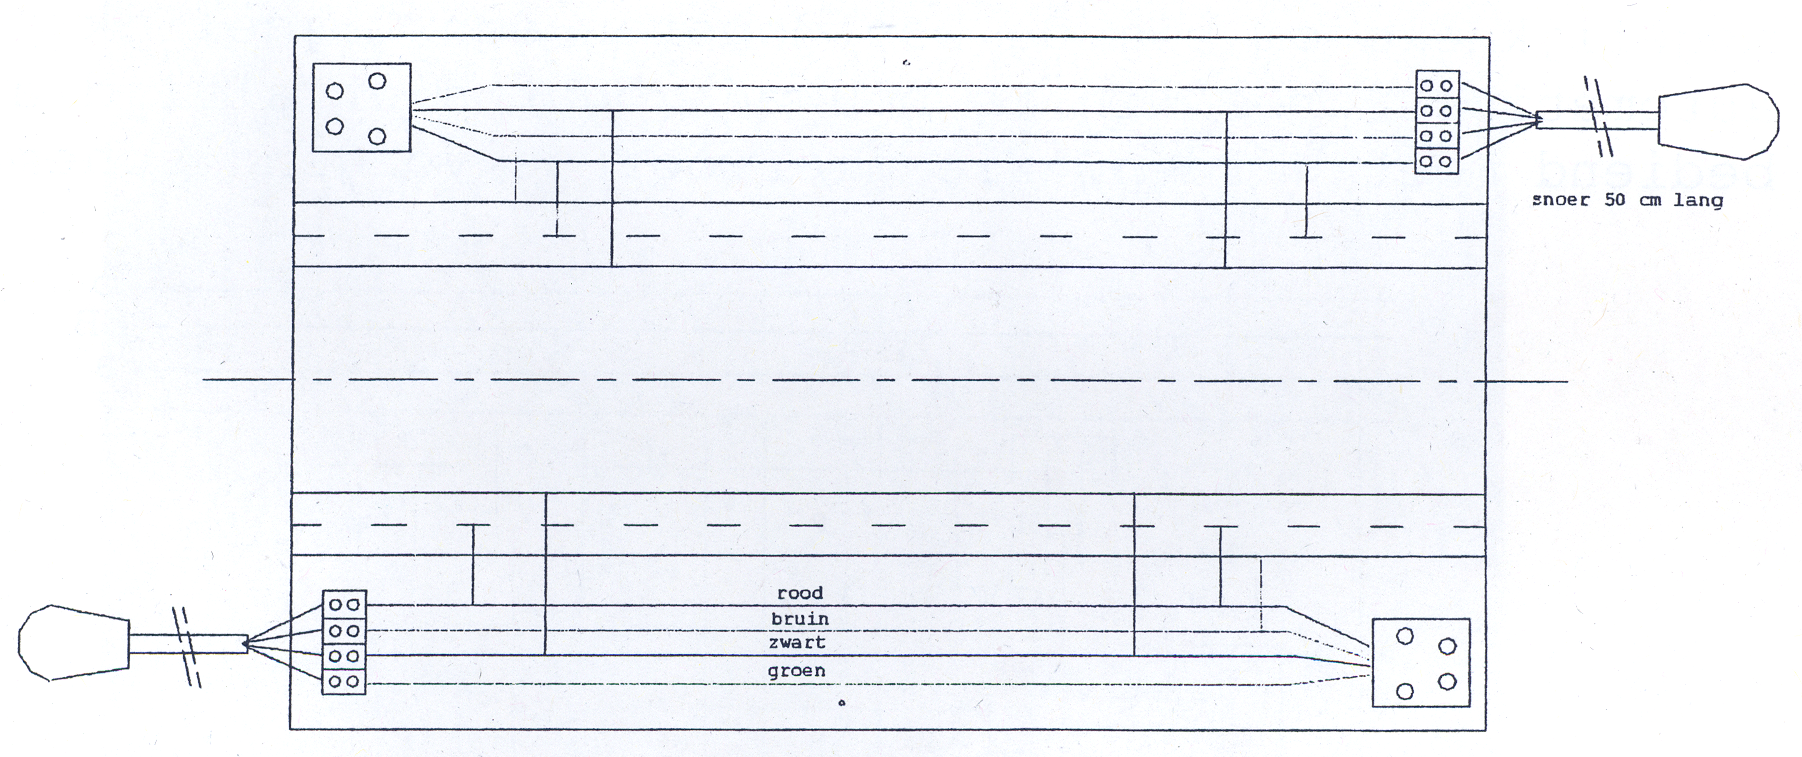
\includegraphics[scale=1.0]{images/rcu_figuur7}

Het is raadzaam om het snoer bij de kroonsteen van een trekontlasting te voorzien, om lostrekken van het snoer uit de kroonsteen te voorkomen.




Het op twee plaatsen aansluiten van de rails per module maakt de installatie bedrijfszekerder. Wanneer er ook in de transformator een beveiliging tegen kortsluiting is ingebouwd, voldoet de installatie aan de voorschriften die bij de vereniging gelden. Dit voorgaande geldt voor zowel gekochte als voor zelfbouw voedingen!


\end{document}


